\documentclass{article}

\usepackage{graphicx}
\usepackage{tikz}
\usepackage{tikzsymbols}
\usetikzlibrary{calc,patterns,shapes.geometric}
\pagestyle{empty}
\usepackage[margin=0pt]{geometry}
\geometry{papersize={14in,12in}}

\def\centerarc[#1](#2)(#3:#4:#5){\draw[#1] ($(#2)+({#5*cos(#3)},{#5*sin(#3)})$) arc (#3:#4:#5);}

\begin{document}
	\begin{figure}
		\centering
		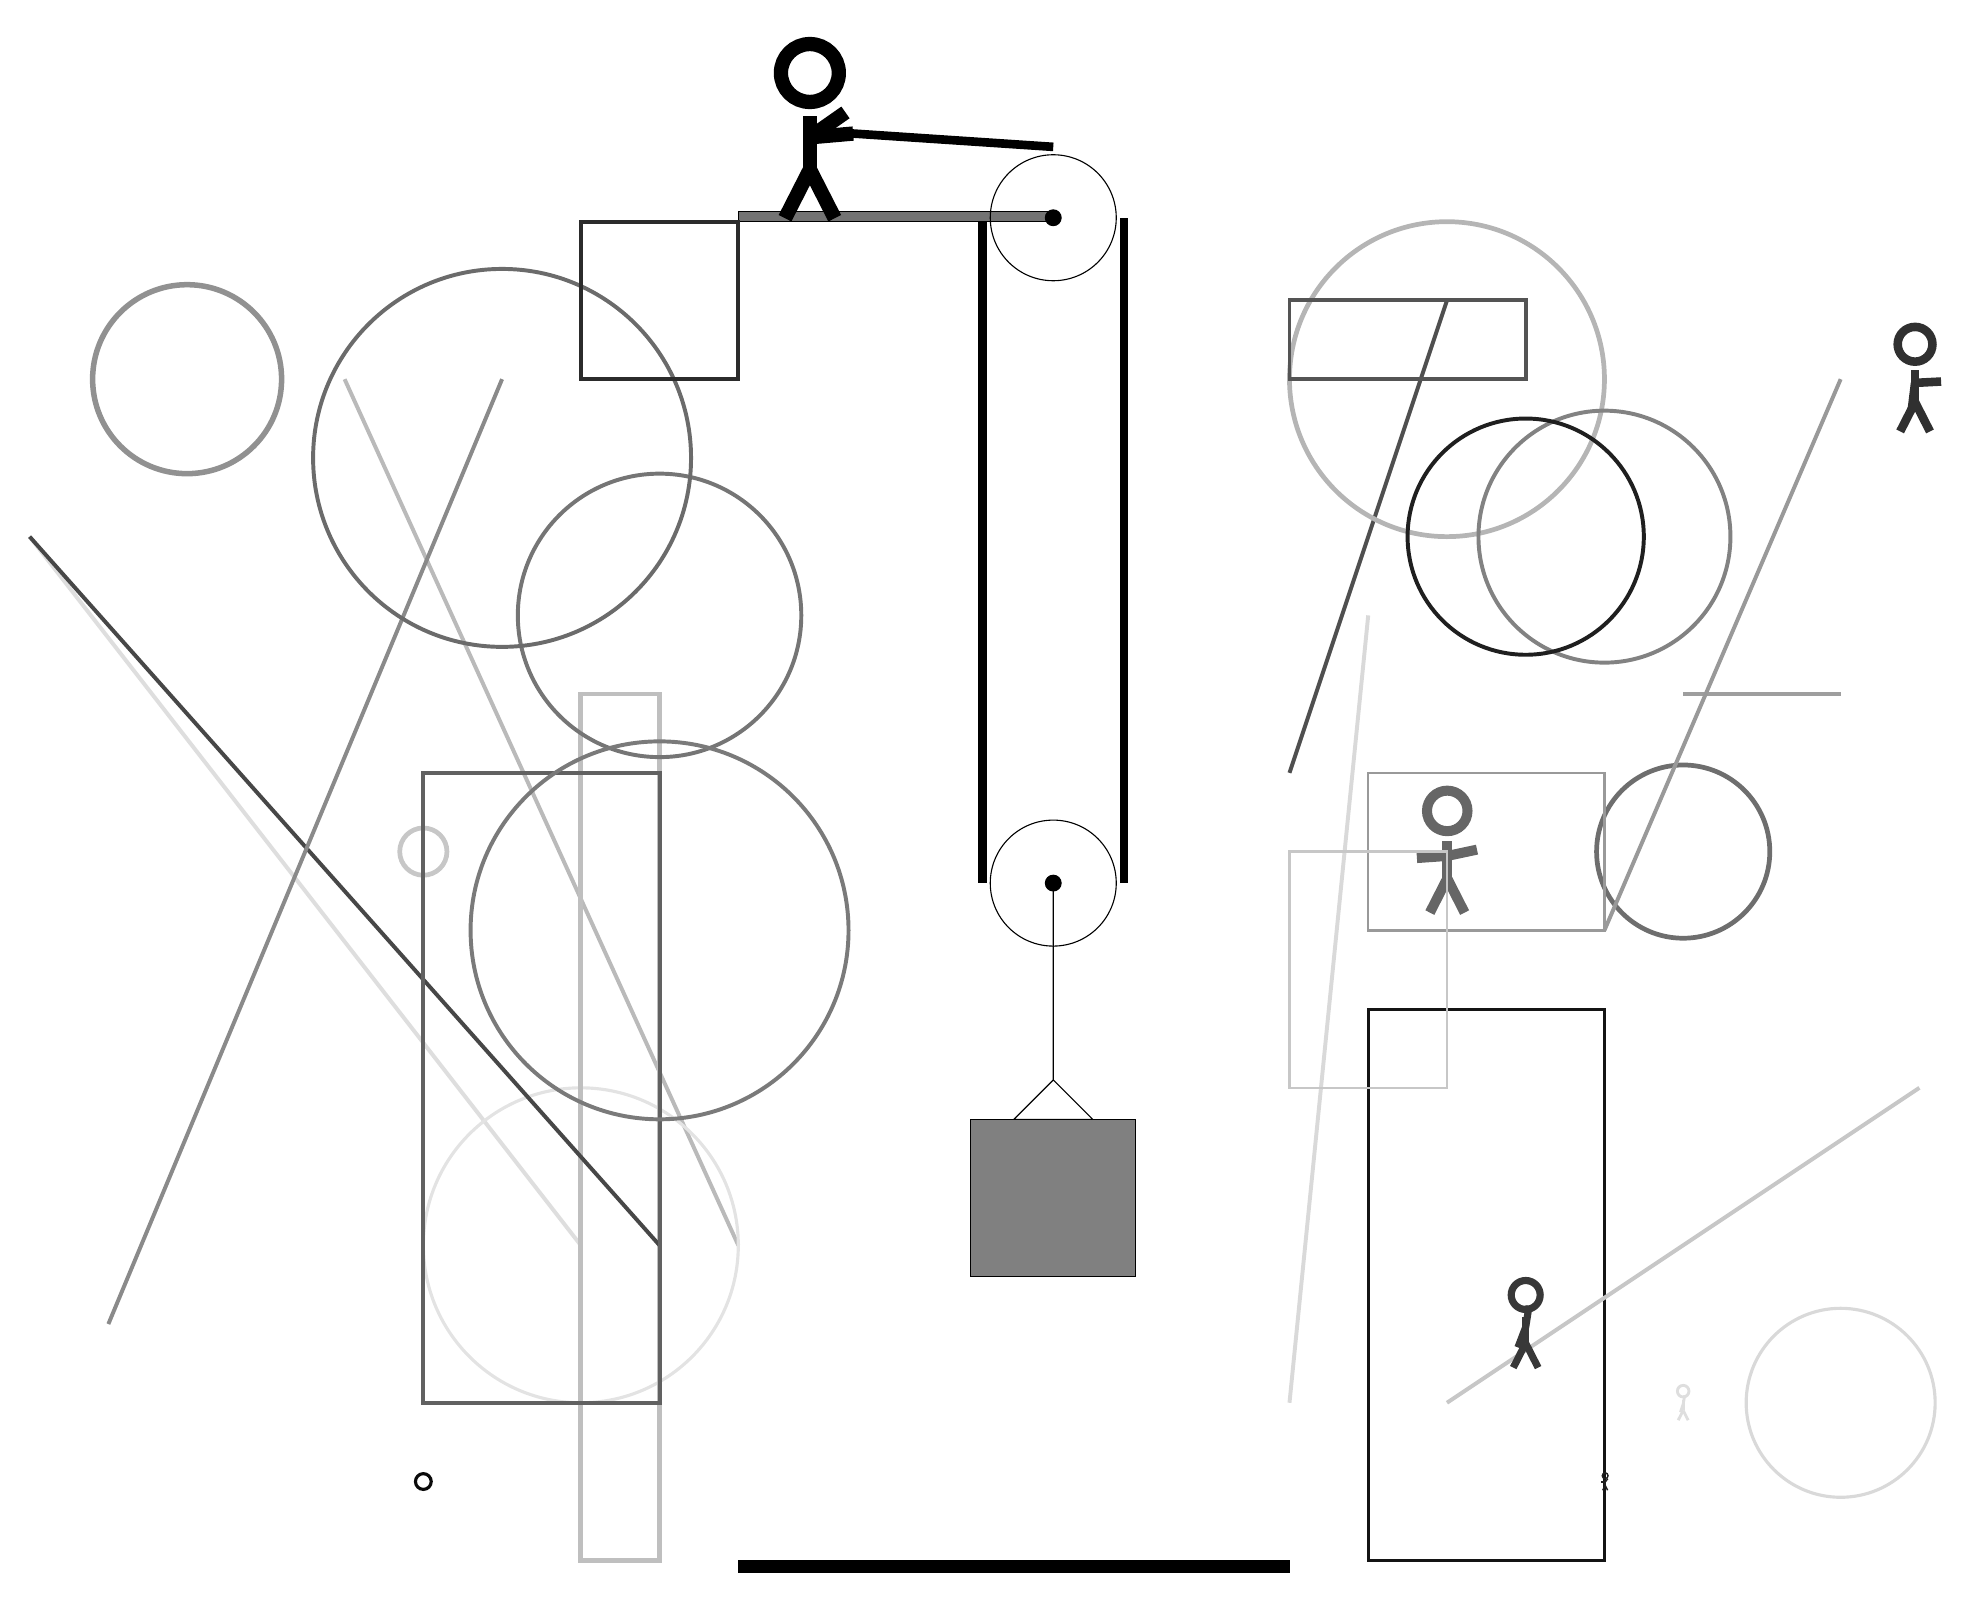
\begin{tikzpicture}
			%%%%% START %%%%%
			
			\draw[fill=black!55] (-2, 14) rectangle (2, 14.125);
			
			\draw[line width=0.4mm, color=black!92] (6, -3) rectangle (9, 4);
			
			\draw [line width=0.4mm, color=black!15](12, -1) circle (1.2);
			\draw[line width=0.5mm, color=black!69](5, 7) -- (7, 13);
			\draw[line width=0.5mm, color=black!13](-4, 1) -- (-11, 10);
			\draw [line width=0.6mm, color=black!29](7, 12) circle (2.0);
			
			\draw[line width=0.5mm, color=black!27](-2, 1) -- (-7, 12);
			
			\draw [line width=0.4mm, color=black!11](-4, 1) circle (2.0);
			\node[line width=0.2mm, color=black!60] at (7, 6) {\Strichmaxerl[7][4][12]};
			\draw[line width=0.5mm, color=black!67] (5, 13) rectangle (8, 12);
			
			\node[line width=0.2mm, color=black!81] at (13, 12) {\Strichmaxerl[6][83][3]};
			\draw [line width=0.4mm, color=black!96](-6, -2) circle (0.1);
			\draw[line width=0.6mm, color=black!25] (-3, 8) rectangle (-4, -3);
			\draw [line width=0.6mm, color=black!57](10, 6) circle (1.1);
			\draw [line width=0.5mm, color=black!49](9, 10) circle (1.6);
			\draw [line width=0.6mm, color=black!22](-6, 6) circle (0.3);
			\draw[line width=0.5mm, color=black!15](6, 9) -- (5, -1);
			
			\draw[line width=0.5mm, color=black!38](10, 8) -- (12, 8);
			
			\draw[line width=0.5mm, color=black!72](-3, 1) -- (-11, 10);
			\draw[line width=0.5mm, color=black!46](-5, 12) -- (-10, 0);
			\draw[line width=0.5mm, color=black!62] (-3, 7) rectangle (-6, -1);
			\draw [line width=0.5mm, color=black!54](-3, 9) circle (1.8);
			\node[line width=0.7mm, color=black!88] at (9, -2) {\Strichmaxerl[1][0][53]};
			\draw[line width=0.5mm, color=black!22](7, -1) -- (13, 3);
			\draw [line width=0.5mm, color=black!58](-5, 11) circle (2.4);
			\draw [line width=0.5mm, color=black!88](8, 10) circle (1.5);
			\draw [line width=0.7mm, color=black!43](-9, 12) circle (1.2);
			
			\node[line width=0.4mm, color=black!13] at (10, -1) {\Strichmaxerl[2][72][80]};
			\node[line width=0.7mm, color=black!78] at (8, 0) {\Strichmaxerl[5][69][81]};
			\draw[line width=0.5mm, color=black!83] (-2, 12) rectangle (-4, 14);
			\draw [line width=0.5mm, color=black!52](-3, 5) circle (2.4);
			\draw[line width=0.3mm, color=black!40] (6, 7) rectangle (9, 5);
			
			\draw[line width=0.5mm, color=black!40](9, 5) -- (12, 12);
			\draw[line width=0.3mm, color=black!22] (7, 6) rectangle (5, 3);
			
			\draw (2, 5.6) circle (0.8);
			\draw[fill=black] (2, 5.6) circle (0.1);
			
			\draw (2, 14.05) circle (0.8);
			\draw[fill=black] (2, 14.05) circle (0.1);
			
			\draw (2, 5.6) -- (2, 3.1) -- (1.5, 2.6) -- (2.5, 2.6) -- (2, 3.1);
			\draw[fill=black!50] (0.95, 2.6) rectangle (3.05, 0.6);
			
			\draw[line width=1.1mm] (1.1, 14) -- (1.1, 5.6);
			\centerarc[line width=1.1mm](2, 5.6)(180:360:0.9);
			\draw[line width=1.1mm](2.9, 5.6) -- (2.9, 14.05);
			\centerarc[line width=1.1mm](2, 14.05)(0:90:0.9);
			\draw[line width=1.1mm](2, 14.95) -- (-1, 15.15);
			
			\node at (-1, 15.15) {\Strichmaxerl[10][-175][35]};
			
			\draw[fill=black] (-2, -3) rectangle (5, -3.15);
			
			%%%%% END %%%%%
		\end{tikzpicture}
	\end{figure}	
\end{document}